\label{chapter:shortestpathmap}

This chapter is dedicated to presenting some formal definition that will help us
precisely discuss the theory in the rest of the thesis. We will also define the
shortest path map and its near relatives the shortest $k$-path map, and some properties
their properties. Finally we will present a Lemma which bounds some complexity of 
the shortest path map which will be usefull later in \ref{chapter:wavefrontpropagation}.

\section{Definitions for shortest paths and shortest $k$-paths}

We start with a trivial definition which we will expand upon.

\begin{mydef}\textbf{Path:}
Given a plane encapsulated by a polygon $\mathcal{P}$, let $s$ and $t$ be two
	points in the plane. We define a path between $s$ and $t$ to be a set of
	vertices and edges which forms a connection from $s$ to $t$.
\end{mydef}

Its trivial to see that a path with a minimum length in the case where $s$ and $t$
are the only entities in the plane will be $\overline{st}$. But we can imagine the
space being occupied not only by two points $s$ and $t$, but also with a set of 
polygons in which a path cannot pass through. We call such polygons obstacles and
we assume through out the rest of this thesis that these obstacles will be 
simple polygons. Since we will represent these with graphs we give a definition of 
simples graphs.

\begin{mydef}\textbf{Simple Graph:}
  A graph is simple if it has no loops and no two of its links join the same pair
  of vertices.
\end{mydef}

Now we might be in a situation where the path with minimum length between two point 
$s$ and $t$ isn't just $\overline{st}$ due to obstacles being placed in the way. We 
further define what space we can create our path in, and which we cannot.

\begin{mydef} 
	\textbf{Free space:}\\ 
	Let $\mathcal{O}=\{O_1,O_2,...,O_k\}$ be a
	family of simple polygons which will act as obstacles in the interior of an
	encapsulating polygon $\mathcal{P}$. We define the free space to be
	$\mathcal{FS}=\mathcal{P}\setminus\mathcal{O}$, that is the plane of the
	encapsulating polygon minus the interiors of all obstacle polygons.
\end{mydef}

The final $O(k^2 \cdot n \log n)$ algorithm that we will be examining will  
need the obstacles to be convex, which are defined as follows: 

\begin{mydef}
	\textbf{Convex Polygons:} \\ 
	A convex polygon is a simple polygon (not self-intersecting) in which no
	line segment between two points on the boundary ever goes outside the
	polygon. In a convex polygon, all interior angles are less than or equal to
	180 degrees, while in a strictly convex polygon all interior angles are
	strictly less than 180 degrees.
	\cite{Bisector-collinearity-convexPoly} 
\end{mydef}

We are only allowed to make paths between $s$ and $t$ in the free space, which we 
will denote as legal paths.

\begin{mydef}
	\textbf{Legal Path:}\\ 
	We define a path between two vertices to be
	legal if it lie entirely in the free space. That is a legal path is disjoint
	from the interiors of all potential obstacle polygons in the plane.
\end{mydef}

Now we are ready to define out legal shortest path between our two points $s$ and 
$t$

\begin{mydef}
	\textbf{Euclidian shortest path:}\\ 
	The legal path of minimum total length connecting the two endpoints is a 
    shortest path.  
\end{mydef}

We define a path which is not legal to be violating, or having a number of
violations, equal to the number of obstacles in which the path will pass
through. We will not only deal with shortest paths which have no violations,
but also shortest path which allow up to $k$ violations.

\begin{mydef}
	\textbf{Shortest k-path}
	The path of minimum total length which violates at most $k$ obstacles.
\end{mydef}

Through out this thesis we will use use the notation of $\pi(s,t)$ to denote the 
shortest paths connecting two points $s$ and $t$ in the case where no obstacle 
violation is allowed. The length of any path in	$\pi(s,t)$ is the shortest path 
distance between $s$ and $t$, denoted $d(p,q)$. If the shortest path between $s$ 
and $t$ is the line segment $\overline{p,q}$, then $p$ and $q$ are said to be 
visible. 

\begin{mydef}
	\textbf{Visibility between points:}
    We define two points $s$ and $t$ to be visible to each other if $s$ and $t$ are 
    connectible with the path $\overline{st}$ which is either legal, or in the case 
    of violations have less that the allowed $k$ violations.
\end{mydef}

The notion of shortest path distance between two sets of points $X$ and $Y$ is 
denoted as $d(X,Y)$ and is the minimum $d(x,y)$ over all pairs of points $x\in X$ 
and $y \in Y$. \cite{HershbergerS99} \\

We call a path violating of at most $k$ obstacles a \textit{$k$-path}, generalizing 
on the traditional obstacle-free path, which is a 0-path. We use the notation of 
$\pi_k(p)$ to be the shortest path in this case where the path can pass through up 
to $k$ obstacles from a \textit{fixed source} $s$ to the point $p$. When reasoning 
about a path with exactly $k$ crossing we denote this as an $(=k)$-path. And 
equally we use $d_k(p)$ to denote the length of the shortest path from the fixed 
source $s$ in the case of up to $k$ obstacle violations. The reason we use a 
separate notation in the case of obstacle violation is that shortest 0-path 
problem with origination at a common source point $s$ cannot intersect, by the 
triangle inequality\cite{HershbergerKS17}

\begin{mydef}
	\textbf{Triangle Inequality:} \\ 
	Let $A$ and $B$ be points in a $\mathbb{R}^n$ space and let $|AB|$ denote
	the distance between $A$ and $B$.  Then the triangle inequality states that
	for three points $A,B,C\in\mathbb{R}^n$ \cite{metricspaceandpoints}
	$$|AB|\leq|AC|+|BC|$$
\end{mydef} 
\begin{figure}[H] 
	\centering
	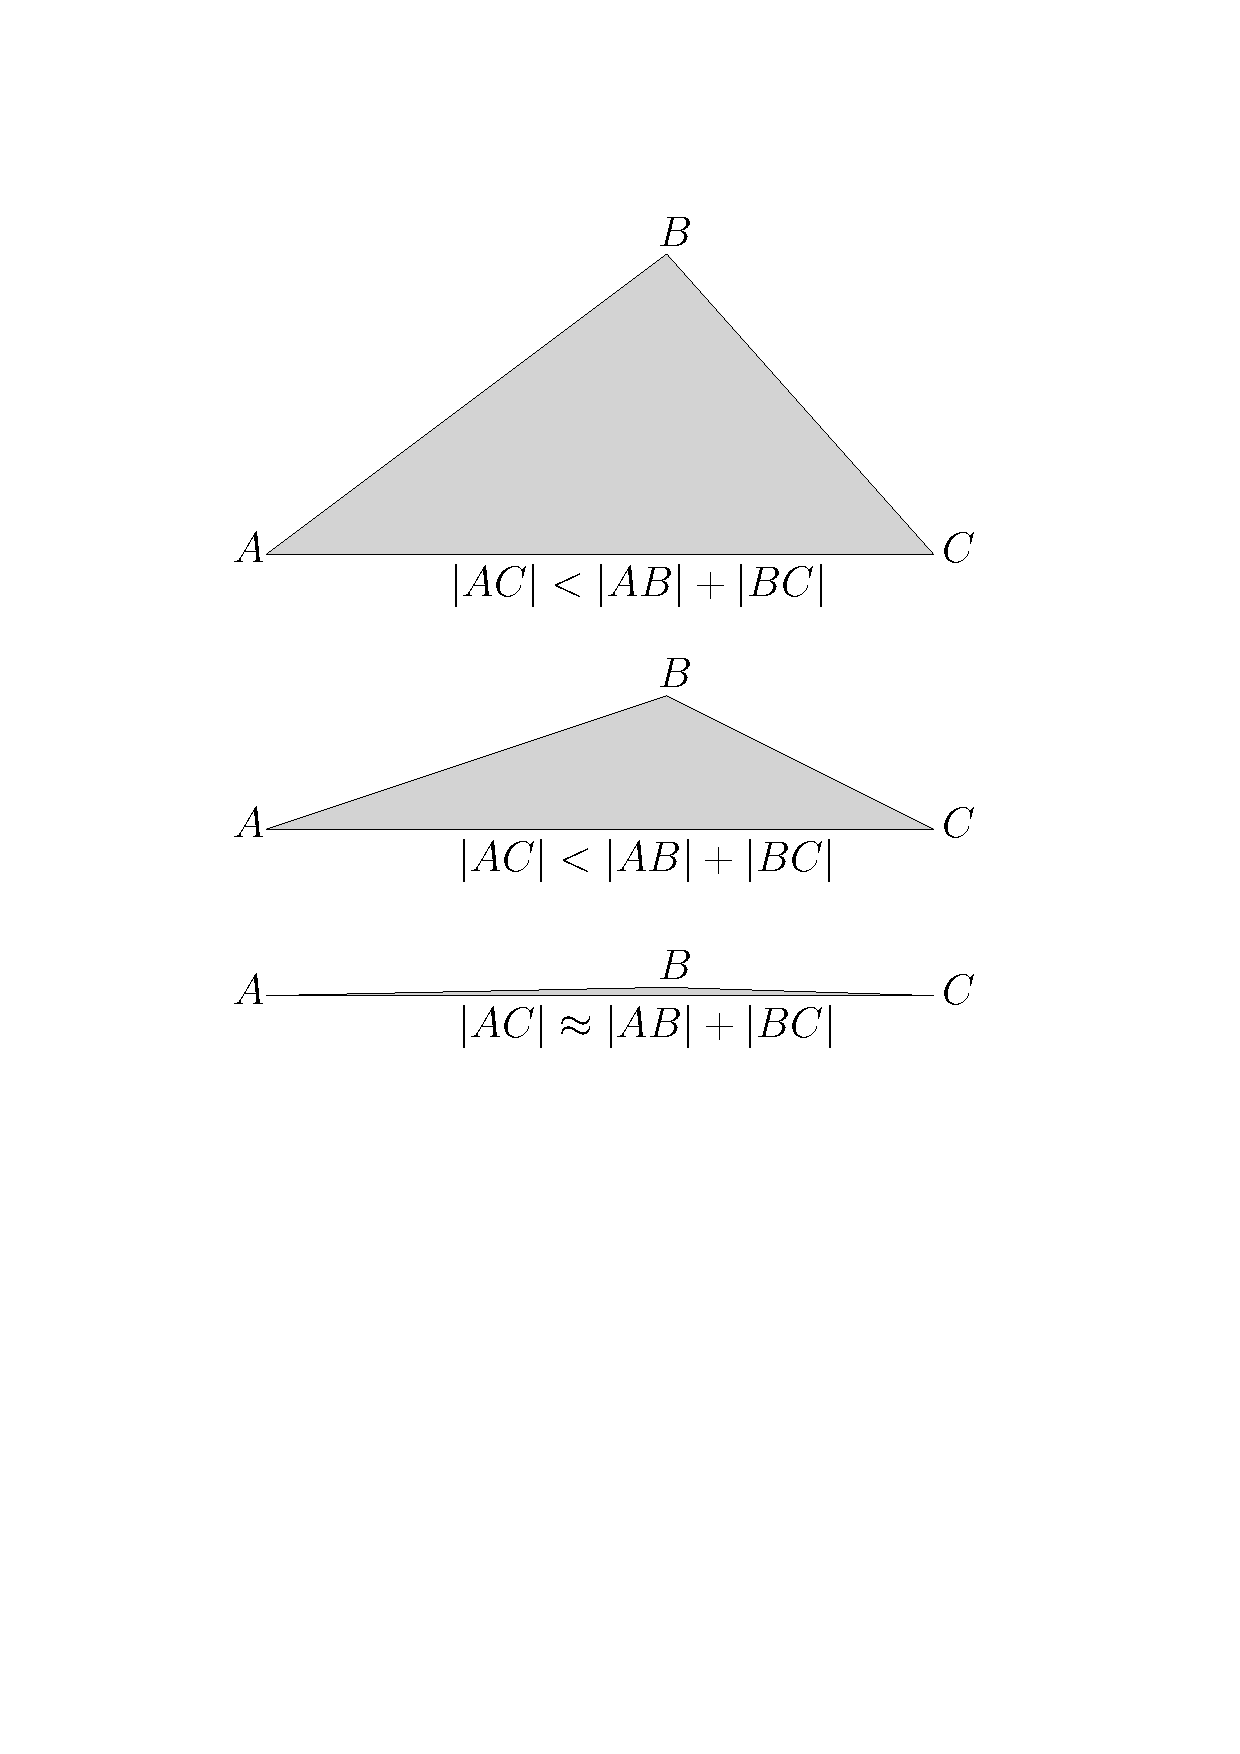
\includegraphics[width=5cm]{figures/TriangularInequality.pdf}
	\caption{Triangular Inequality approaching equality}
	\label{fig:TriangularInequality} 
\end{figure}


\section{Shortest path map and shortest $k$-path map}

This section will briefly introduce the reader to the concept of shortest path map
and shortest $k$-path map and som basic properties of these.

We begin this section with a definition of a predecessor which is essential to understand
what a shortest path map is

\begin{mydef}
	\textbf{Predecessor:} \\ 
	The predecessor of an arbitrary point $p$ is defined as a vertex in the plane which is 
	adjacent to $p$ in $\pi(p,s)$. These vertices also include the source $s$. A predecessor of
	$p$ is necessarily visible from $p$. If $p$ and $s$ are mutually visible,
	then $s$ is a predecessor of $p$. \cite{HershbergerS99} 
\end{mydef}

next we give the definition of a shortest path map

\begin{mydef}
	\textbf{Shortest Path Map:} \\ 
	The shortest path map  of a
	particular source point s, denoted $SPM(s)$, is a subdivision of the plane
	into two-dimensional regions such that all the points in one region have the
	same, unique predecessor\cite{HershbergerS99}. 
\end{mydef}

An example of an $SPM$ can be seen in figure \ref{fig:exampleofspms} blow

\begin{figure}[H] 
	\centering
	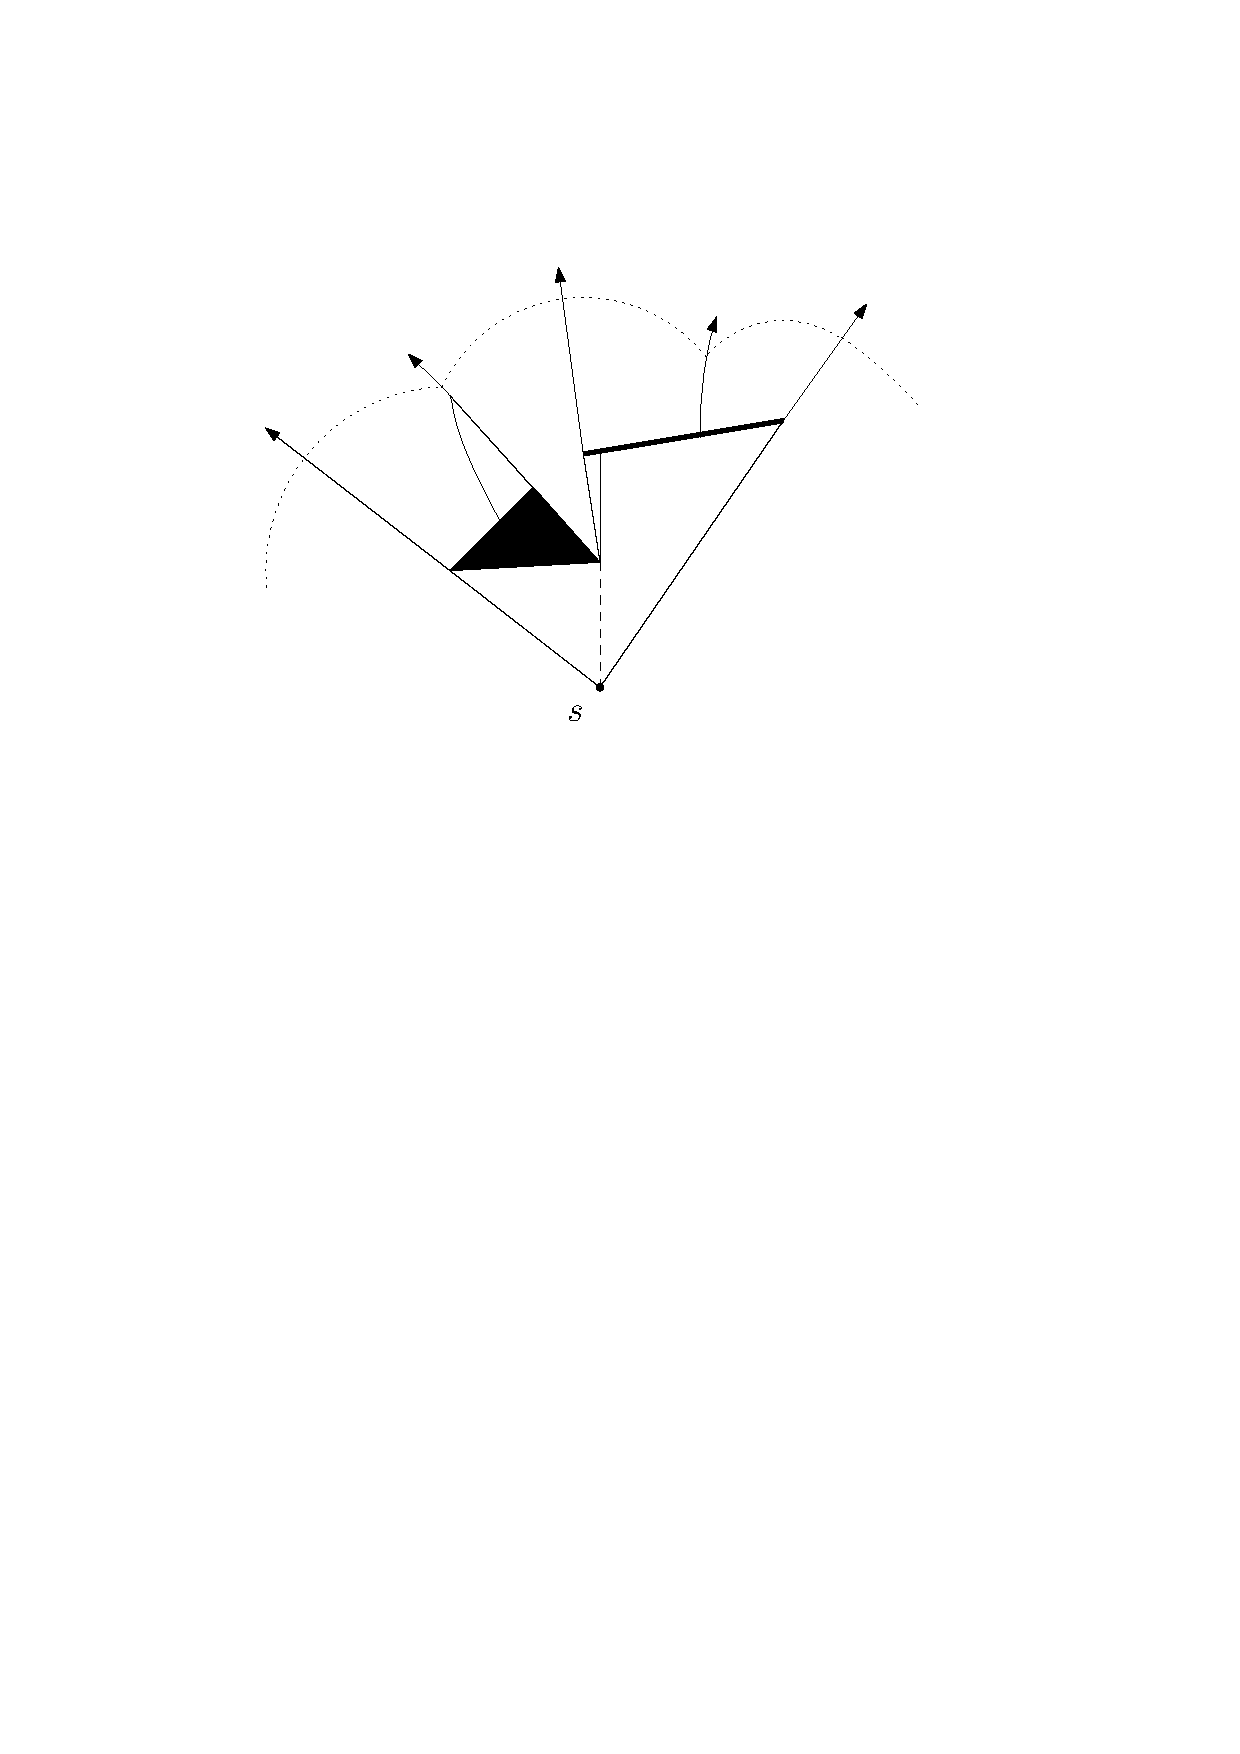
\includegraphics[width=0.65\textwidth]{figures/exampleofspms.pdf}
	\caption{An example of an $SPM$ build around $s$ with where the area between
	         the arrows and fully drawn lines shows the regions in the plane with
	         the same predecessors.}
	\label{fig:exampleofspms} 
\end{figure}

The figures shows the $SPM$ build around $s$ as the source, and the different obstacles in the plane. 
Since a shortest path only needs to turn at the vertices of the obstacles, by triangular inequality, 
the vertices of obstacles naturally constitute the unique predecessors of the points within the different 
regions marked by the fully drawn lines. Here the lines will extend until the meet the encapsulating 
polygon $\mathcal{P}$ an then be fully enclosed. The dashed lines show the shortest path from a region 
$s$ or to the preceding region. It should be noted that these fully drawn line constitutes bisectors 
(which will explained in later chapter) and there point on the line have a equal distance to $s$ through 
either of the regions which the bisector acts a border between. It should therefore be noted that in the 
case of the $SPM$ there may multiple shortest paths to points in the plane, in which case one just chooses 
one of them.

The distance to a point $p$ in the $SPM$ is calculated by finding the weight from $s$ to $p$

\begin{mydef}
	\textbf{Weight:} \\ 
	We define weight of an vertex (including obstacle vertices) to be
	its shortest path distance to the source $s$. Given an arbitrary point $p$
	in free space, its weighted distance to a visible vertex $v$ is defined as
	$$d(s,v) + \left| \overline{vp} \right|$$
	that is the straight-line distance from $v$ to $p$ plus the shortest path 
	distance from $s$ to $v$.
	\cite{HershbergerS99} 
\end{mydef}

Next we move on to the definition of $k$-predecessors and the shortest $k$-path map

\begin{mydef}
	\textbf{$k$-predecessor}\\ 
	Given a shortest $k$-path $\pi_k(p)$, we define the \textit{predecessor of
	p} to be the vertex (including $s$) that is adjacent to $p$ in
	$\pi_k(p)$\cite{HershbergerKS17}. 
\end{mydef}

\begin{mydef}
	\textbf{Shortest k-path map}(Definition 9 in \cite{HershbergerKS17})\\
	The partition of free space into connected regions with the same
	$k$-predecessor is called the \textit{shortest k-path map}, and is denoted
	by $SPM_k$. The subset of $SPM_k$ for which the shortest path $\pi_k(p)$ to
	every point $p$ has exactly $k$ crossings is called the shortest $(=k)$-path
	map and denoted by $SPM_{=k}$. 
\end{mydef}

It is quite easy to see that a $SPM$ is the same as an $SPM_{=0}$, we will therefore use $SPM$ when 
dealing with the Hershberger-Suri algorithm in chapters \ref{chapter:conformingsubdivision} and 
\ref{chapter:wavefrontpropagation}, and $SPM_{=0}$ when dealing with the computing of $SPM_k$ in
chapter \ref{chapter:shortestpathobstaclesviolation}.

We saw with the $SPM_0$ map that each predecessor to an region always where on the boundary on said
region, this isn't necessarily the case for a $SPM_k$. Further more multiple regions in $SPM_k$ may 
have the same predecessor see figure \ref{fig:1predecessor}.

\begin{figure}[H] 
	\centering
	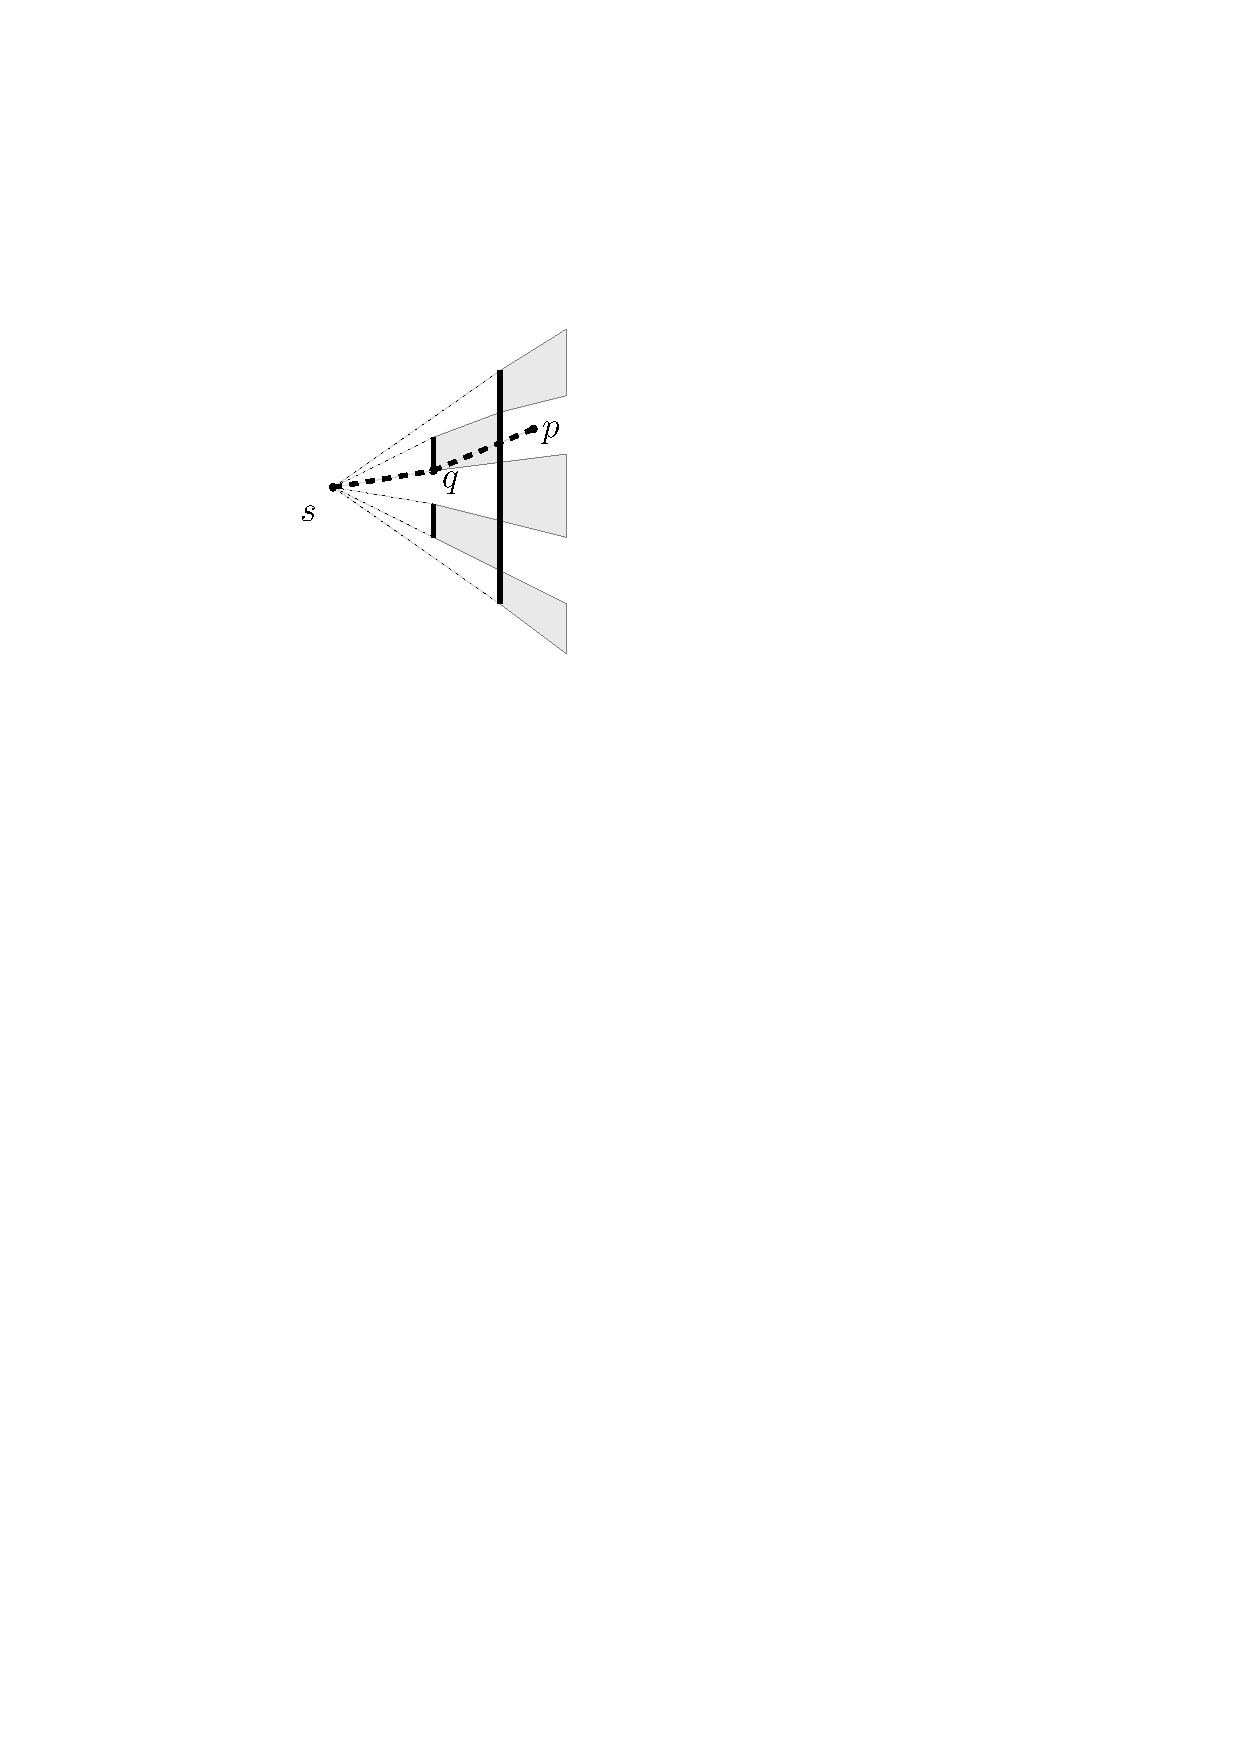
\includegraphics[width=0.4\textwidth]{figures/1predecessor.pdf}
	\caption{Here we present a $SPM_1$ map, where we the fat lines are obstacles.}
	\label{fig:1predecessor} 
\end{figure}

Here we see that the shortest path from $s$ to $p$ goes through point $q$ which lies outside the region
in which $p$ is. So we need to maintain additional information with polygon vertices to disambiguate the 
predecessor relation. So suppose we have a live segment $\overline{vp}$ between to vertices which crosses
$(k-1)$ obstacles for some $0 \leq i \leq k$, then the length $d_k(p)$ of $\pi_k(p)$, is defined as
the sum of the length of the $i$-path to $v$ and the length of segment $\overline{vp}$. So in the context
of figure \ref{fig:1predecessor}  we have $\overline{qp}$ crosses $(k-1)$ obstacle in the relation of $0 \leq
1 \leq k = 1$, which leaves the $k - 1 = 0$ obstacles left which we can cross. The $0$-path to $q$ is the
direct path $\overline{sq}$, where we have the total shortest path.

So for a point $p$ in $SPM_{=k}$, we identify the $k$-predecessor of $p$ by the pair $(v,i)$, where $v$
is a vertex of $\mathcal{P}$ and $i \in \{0,1,..,k\}$ such that $d_k(o) = d_i(v) + |\overline{vp}|$ and the
segment $\overline{vp}$ crosses $(k-i)$ obstacles \cite{HershbergerKS17}.

Neat property of the $SPM_k$ is we devide it into two parts, a $V_{k-1}$ path which is the region consisting of
$k-1$-visible points, which is starshaped, and the $SPM_{=k}$ part. The concept of $V$ areas can be seen in
figure \ref{fig:regions}.

\begin{figure}[H] 
	\centering
	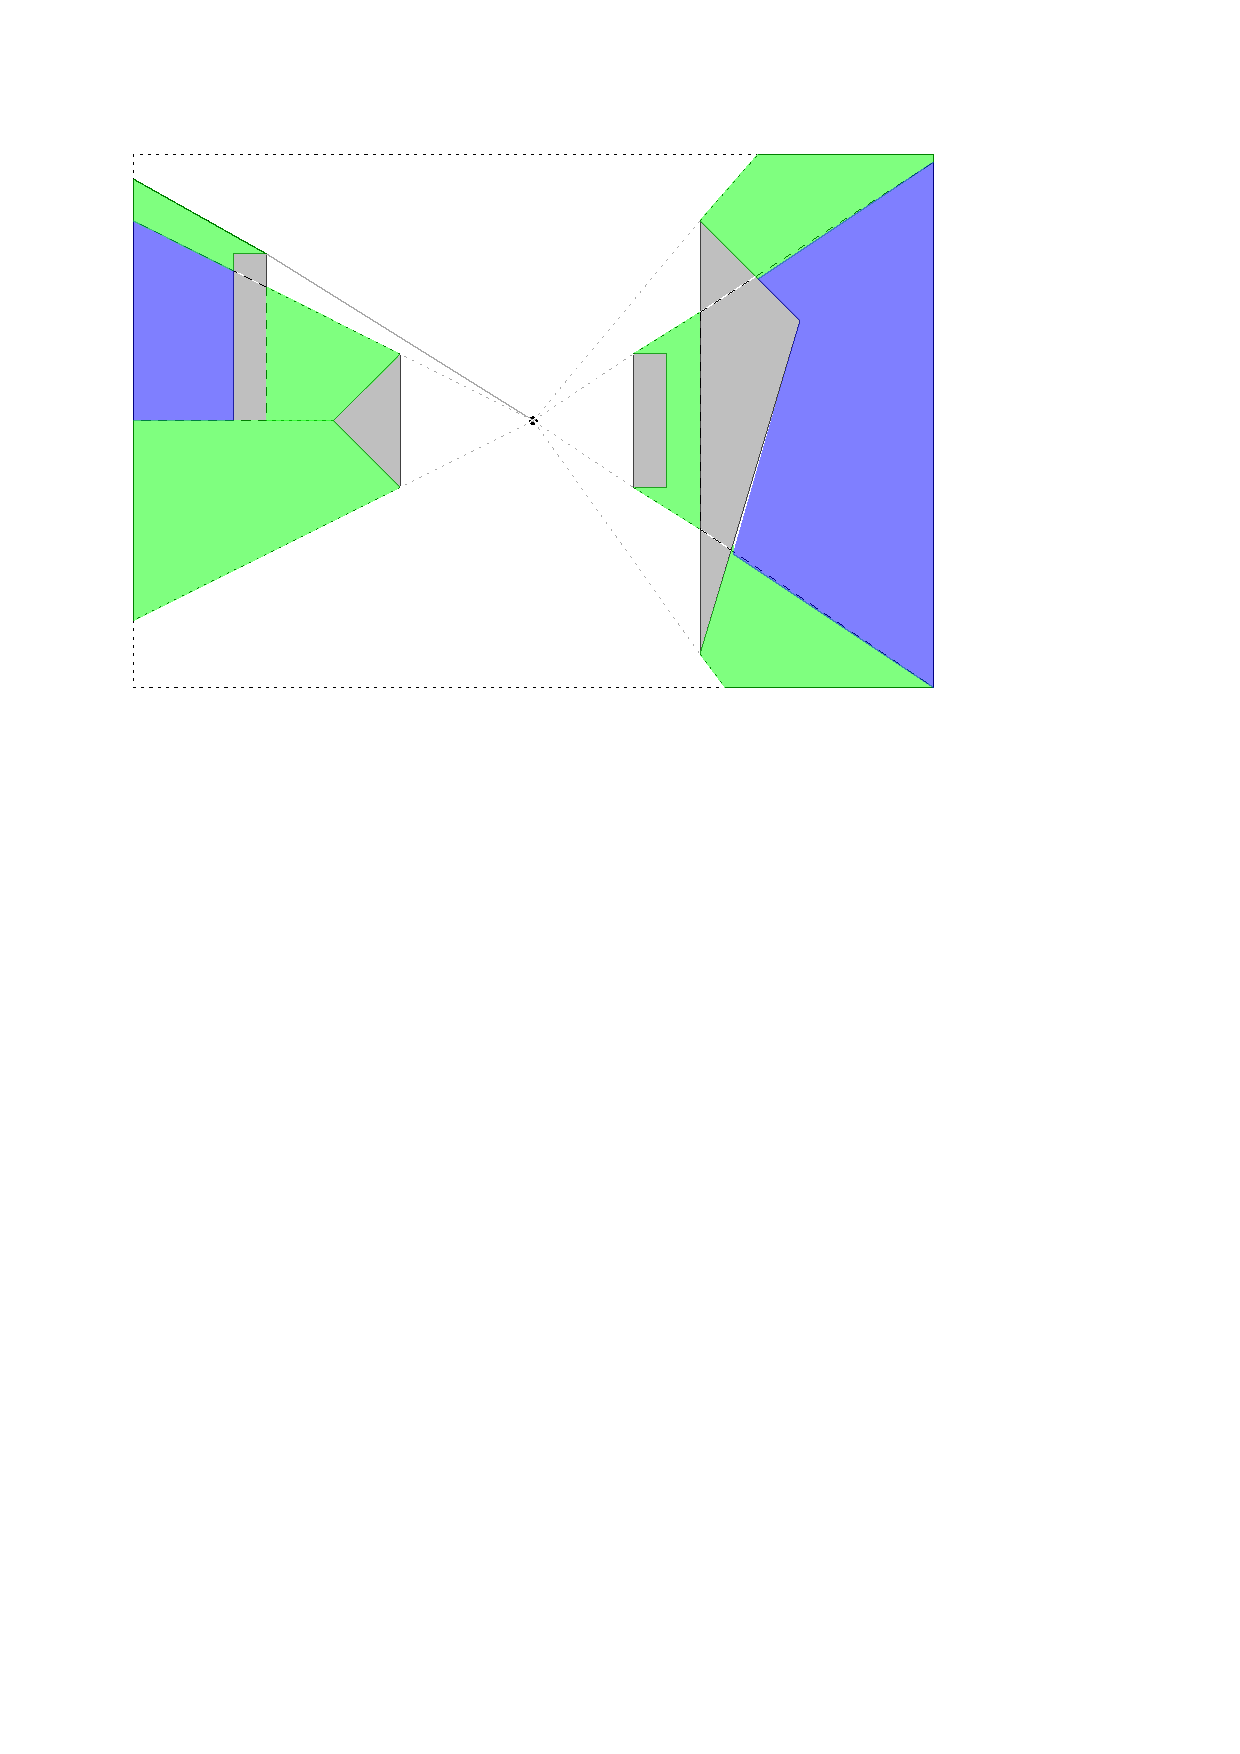
\includegraphics[width=0.8\textwidth]{figures/regions.pdf}
	\caption{Here the boundary of $V_1$ is marked with dashed lines, while the region of $V_0$ is shown with 
	         dotted lines. $V_1$ is further shown with blue and the $V_1 \setminus V_0$ is shown with green.}
	\label{fig:regions} 
\end{figure}

\section{Complexity of $SPM$ map}

Here follows a Lemma which will be usefull for bounding the number of hyperbolic arcs in the proof 
of Lemma \ref{lemma:4.12} in chapter \ref{chapter:wavefrontpropagation} but first we define what
a star-shaped polygon is.

\begin{mydef}[Star-shaped polygon]\cite{PreparataS85}
	\label{star-shaped}
	A simple polygon $P$ is star-shaped if there exists a point $z$ not external
	to $\mathcal{P}$ such that for all points $p$ of $\mathcal{P}$ the line segment 
	$\overline{zp}$ lies entirely within $P$. The locus of the points $z$ having the 
	above property is the \emph{kernel} of $\mathcal{P}$.
\end{mydef}

\begin{Lemma}[Lemma 3.2]
	\label{lemma:3.2}
	The shortest path map $SPM(s)$ has $O(n)$ vertices, edges and faces. Each
	edge is a segment of a line or a hyperbola
\end{Lemma}
\begin{proof}
	Note that each face $SPM(s)$ is star-shaped (see definition
	\ref{star-shaped})
	with the unique predecessor vertex for the face, and the predecessor is in
	the kernel of the face.
	The idea behind this proof is to show that each obstacle vertex is a
	predecessor vertex for at most one face in $SPM(s)$.
	Consider a vertex $u$ that is the predecessor of a face $F$ and let
	$pred(u)$ be the set of predecessors of $u$, this is a set because there can
	be multiple predecessors. Observe that $d(s,u)=d(s,v)+|\overline{uv}|$ for
	any $v\in pred(u)$, since the distance $d(s,u)$ can always be rewritten as
	the distance to from $s$ to $u$'s predecessor, and a straight line from the
	predecessor to $u$ since your predecessor is always visible from a point.

	If a point $p$ is visible from a vertex $v \in pred(u)$ with $v$, $u$, $p$ 
    not being collinear, then $p$ cannot have $u$ as its predecessor. This is 
    due to the triangle inequality, where it is always shorter to take the direct 
    line instead going by another point.


	Consider the subset of the free space that is visible from $u$
	but not visible from $v\in pred(u)$. Let $R(u,v)$ denote the component of
	this subset that is incident to $u$. Then $R(u,v)$ lies in an
	angular angle around $u$ of less than 180$^\circ$. Define
	\begin{align}
		R(u) =  \bigcap_{v\in pred(u)} R(u,v)
	\end{align}

	Clearly $F \subseteq R(u)$, since the area $R(u)$ is the area that is
	incident to $u$, and not visible from any predecessor $v\in pred(u)$ 
	
	Then the claim is that there is at most one face of
	$SPM(s)$ in $R(u)$ with $u$ as its predecessor. 
	
	We do this by contradiction: 
	Suppose there were two faces
	$F_1$ and $F_2$ both having $u$ as their unique predecessor. The faces $F_1$
	and $F_2$ must have exactly one point in common, the vertex $u$. In the space
	between $F_1$ and $F_2$ there is a point $p$, there have to be a point here,
	otherwise they would be the same face. The point $p$ is arbitrarily close to $u$ with
	predecessor $z$ such that $z$ is distinct from both $u$ and $pred(u)$. In
	other words $d(s,u)+|\overline{up}|>d(s,z)+|\overline{zp}|$. However as $p$
	moves towards $u$ the difference in the distance shrinks and finally
	$d(s,u) = d(s,z)+|\overline{zu}|$. But then $z$ must be a predecessor of
	$u$. This means that $F_1$ and $F_2$ is part of the same face, contradicting
	the hypothesis. Thus a vertex $u$ is a predecessor of at most one face in
	the shortest path map.

	Finally to prove the linear upper bound on the size of the shortest path
	map, recall that the number of obstacle vertices is $n$ the remaining
	vertices border at least three faces of $SPM(s)$ (for this argument we count
	the obstacle polygons as faces of the shortest path map). Since the number
	of faces is $O(n)$, Eulers formula for planar graphs implies that the total
	number of vertices is also $O(n)$. This completes the proof
\end{proof}
